\section{Recording CPU Load}
\label{sec:qstat}

Recording the CPU load is executed by a self-programmed tool of Michael Iedema (michael\@askozia.com). Its name is
\texttt{qstat} and is available by pressing the \texttt{ESC} key somewhere on the Askozia webpage. Then, in the
``Beta Features'' tab, there is a link referencing to \texttt{debug\_qstat.php}:

\begin{figure} [!ht]
\centering
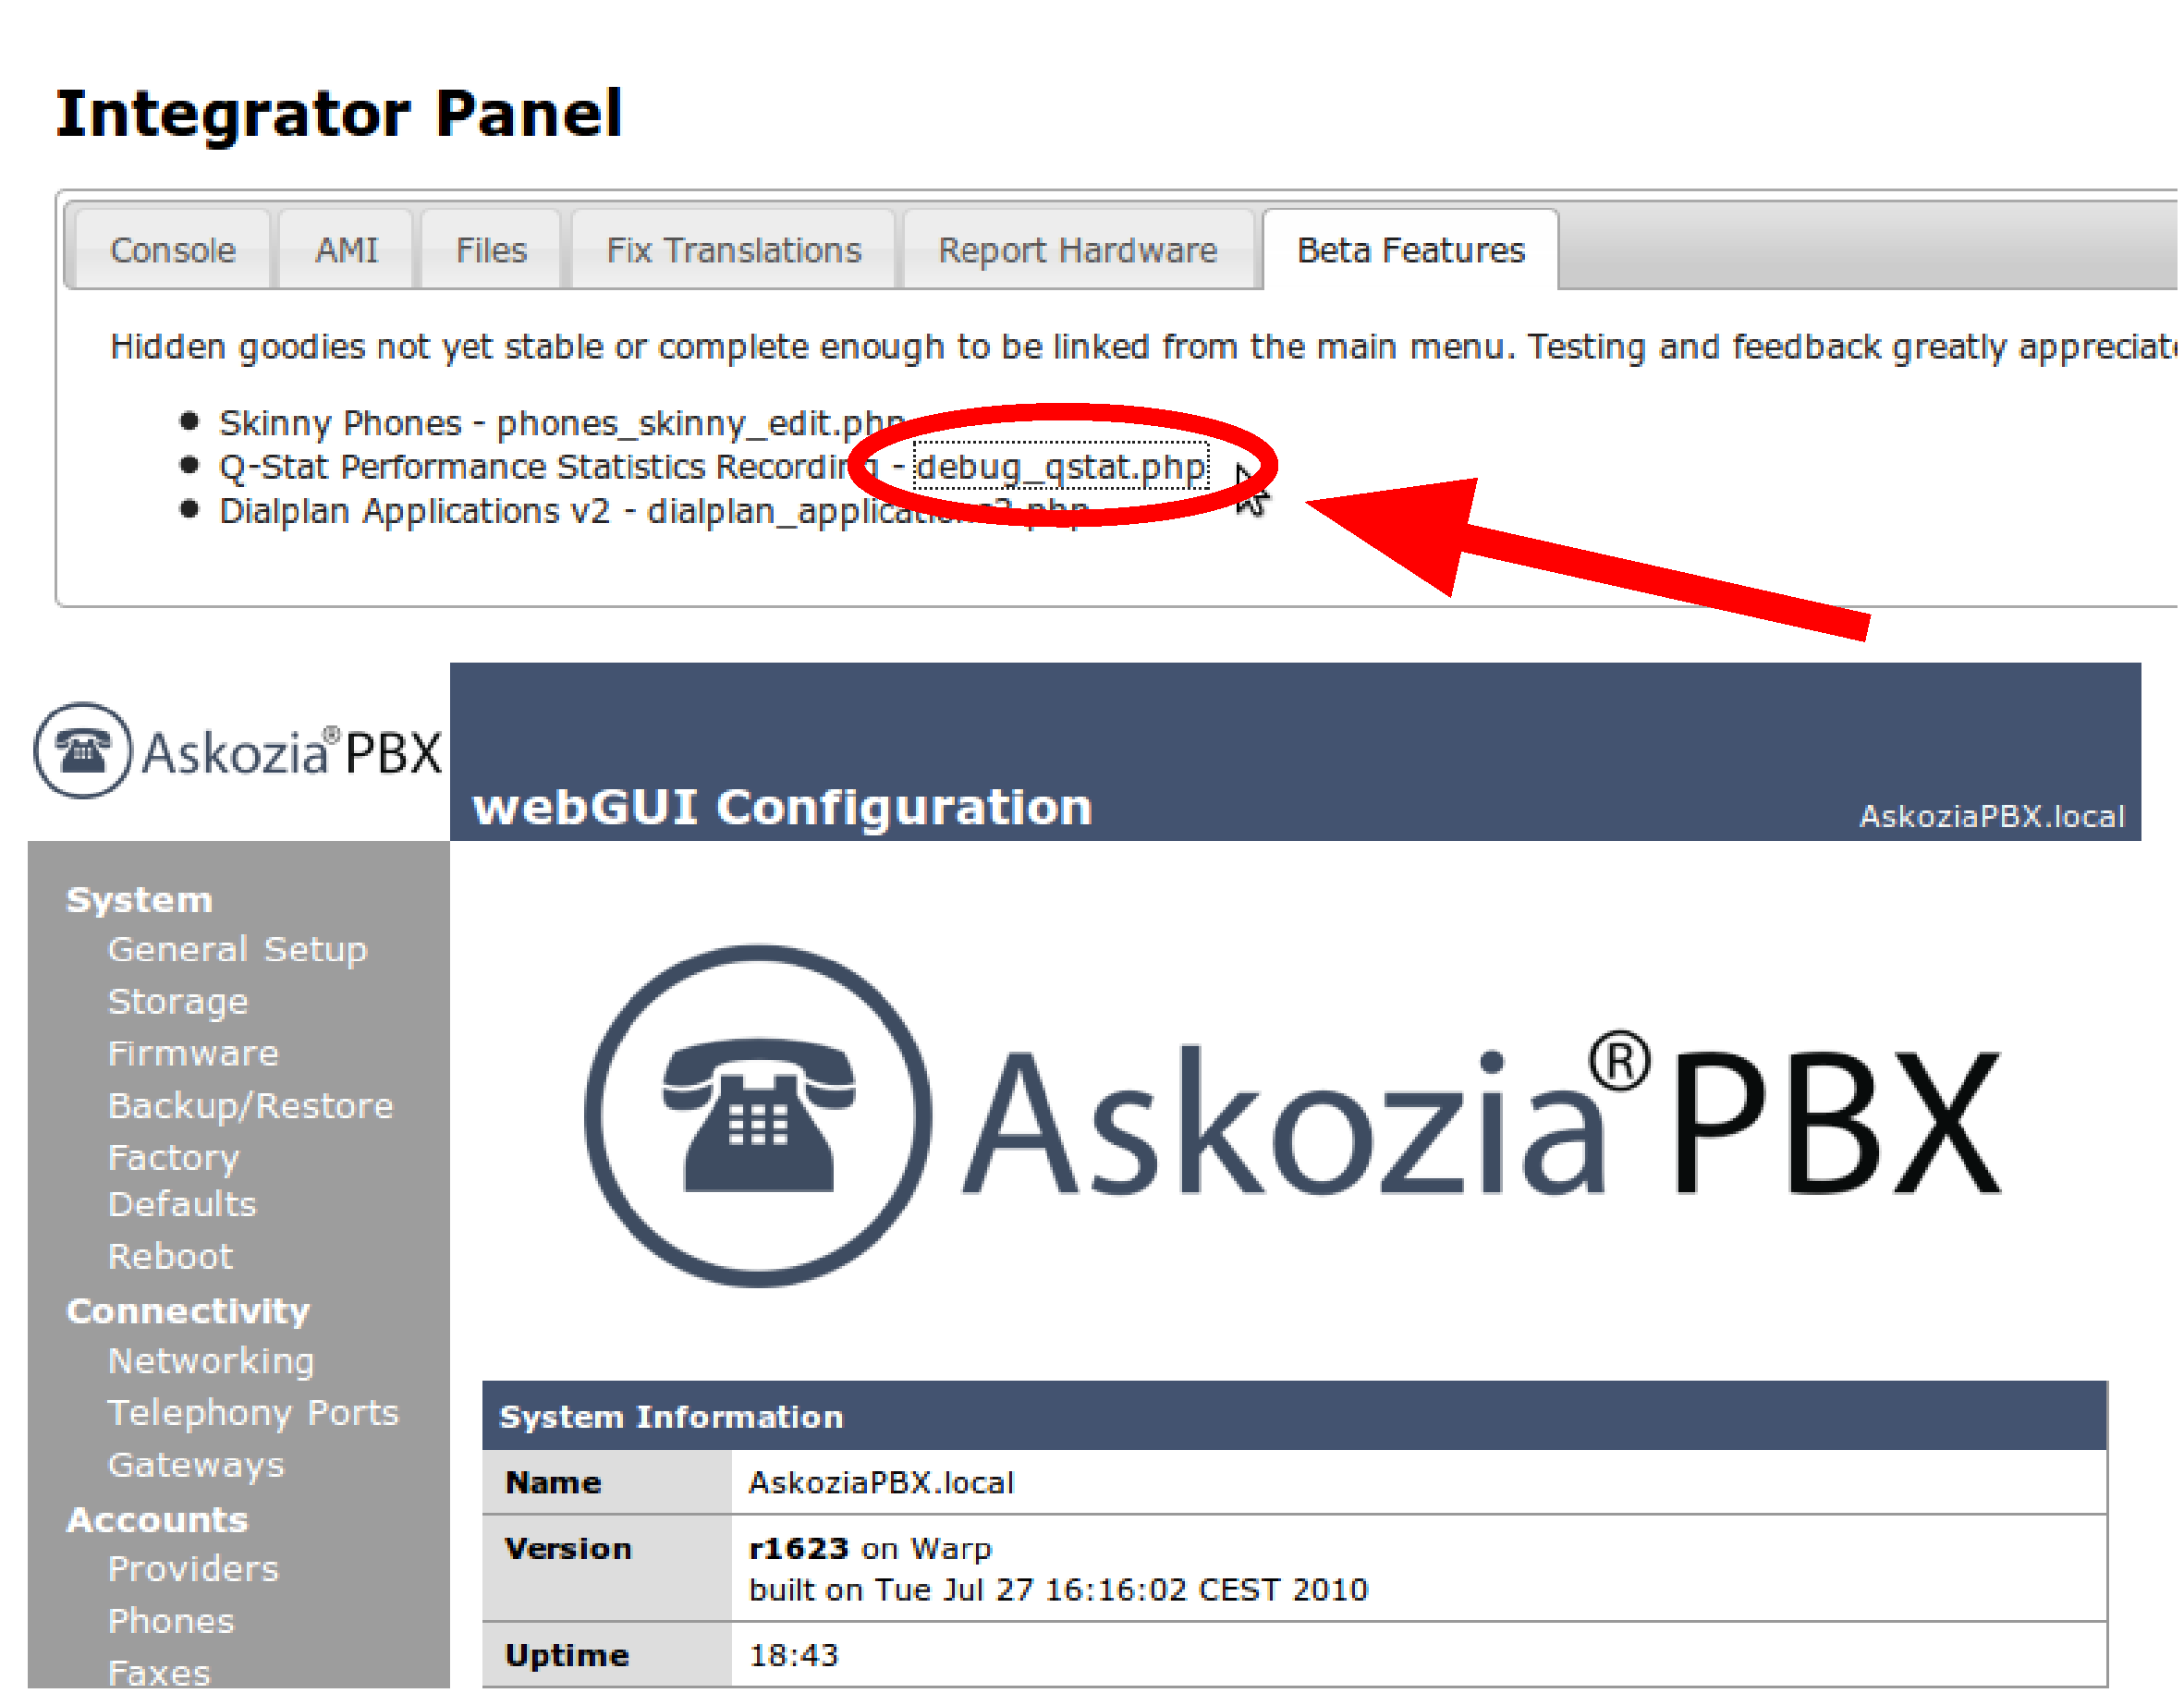
\includegraphics [width=16cm] {qstat-1.pdf}
\caption{Starting qstat manually}
\end{figure}

On the debug qstat page, there is only one button labelled with \texttt{Start}. So, a click on this button starts CPU load
recording by qstat. The button changes top \texttt{Stop} automatically and terminates CPU load recording by clicking on it.
After this, there appears a downloadable file (... .qstat) on the webpage. It contains the recorded qstat data and looks like this:

\begin{figure} [!ht]
\centering
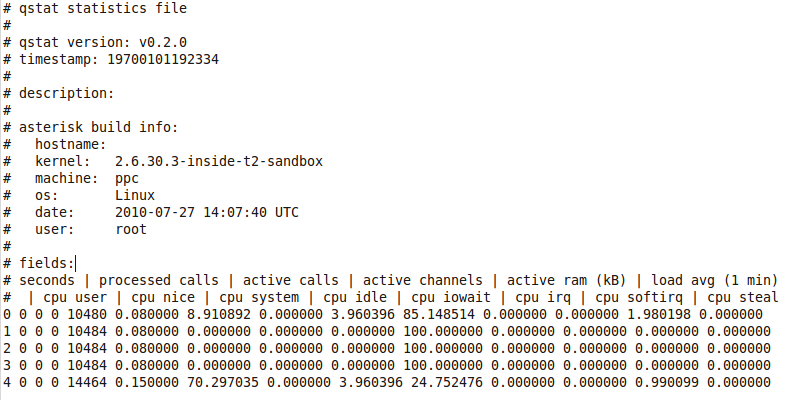
\includegraphics [width=17cm] {qstat-2}
\caption{QStat results}
\end{figure}

The recorded data comprise multiple CPU load values. The script uses the CPU idle time by subtracting it from 100. They were
verified by using \texttt{top} on the AskoziaPBX.
